\documentclass{article} % For LaTeX2e
\usepackage{iclr2015,times}
\usepackage{hyperref}
\usepackage{url}
\usepackage{subfigure}
\usepackage{graphicx}

\title{Deep learning vector quantization}

\author{
Harm de Vries\\
Universit\'{e} de Montr\'{e}al\\
\texttt{mail@harmdevries.com} \\
}

% The \author macro works with any number of authors. There are two commands
% used to separate the names and addresses of multiple authors: \And and \AND.
%
% Using \And between authors leaves it to \LaTeX{} to determine where to break
% the lines. Using \AND forces a linebreak at that point. So, if \LaTeX{}
% puts 3 of 4 authors names on the first line, and the last on the second
% line, try using \AND instead of \And before the third author name.

\newcommand{\fix}{\marginpar{FIX}}
\newcommand{\new}{\marginpar{NEW}}

%\iclrfinalcopy % Uncomment for camera-ready version

%\iclrconference % Uncomment if submitted as conference paper instead of workshop

\begin{document}


\maketitle

\begin{abstract}
We propose to replace the traditional softmax and cross entropy loss in deep neural networks with Generalized Learning Vector Quantization, an efficient prototype based classifier. 
\end{abstract}

\section{Introduction}



\section{Generalized Learning Vector Quantization}
We assume we are given training data $(\mathbf{x}^{(n)}, y^{(n)}) \in R^D \times \{0, ..., K-1\}$, $n=1, .... N$, where $D$ is the dimensionality of the input, and $K$ the number of classes. A LVQ classifier consist of a set of prototypes ${\mathbf{w}_j} \in R^D, j=1, ..., M$ with an associated class label $c(w_j) \in \{1, ..., K\}$. In this work we consider one prototype per class, although ordinary GLVQ often requires multiple prototypes per class to account for multiple modes in the input space. Classification takes place by a nearest prototype scheme i.e. a new data point $\tilde{x}$ is assigned to the class of the nearest prototype $c(\mbox{arg min}_j d(\tilde{x}, \mathbf{w}_j))$ according to some distance measure $d(\tilde{x}, w_j)$. Throughout the following we consider the Euclidean distance $d(\tilde{x}, w_j) = \|x - w_j\|_2$ but other differentiable distance measures can be used. 

Training aims to find the locations of the prototypes such that the data points are mapped to their corresponding class labels. Generalized Learning Vector Quantization (GLVQ) \cite{sato1996generalized} aims to achieve this by minimizing the following training criterion:
\begin{equation}
 L_{GLVQ}(\theta) = \sum_i \phi\left(\frac{d^+ - d^-}{d^- + d^+}\right)
\end{equation}
where $d^+ = \mbox{min}_{c(w_j) = y} d(x^{(n)}, w_j)$ and $d^- = \mbox{min}_{c(w_j)\neq y} d(x_i, w_j)$ denote the distance to the closest correct and closest wrong prototype, respectively. The numerator denotes the margin between the correct and wrong class, while the denominator scales the term within the interval $[-1, 1]$. The complete term is negative when a data point is correctly classified. The scaling function $\phi$ provides a handle to balance error minimization and margin maximization. Using the step function corresponds to the non-differentiable zero-one loss, and using the identity function corresponds to an average margin maximization. Often, a trade-off between the two terms is achieved by a scaling function $\phi(x) = \exp(\gamma x)$, where $\gamma > 0$ controls the steepness of the exponential. 
There are two other important observation to make about the cost function: 
\begin{itemize}
\item The loss is invariant to the scale of the distances. That is, if each distance is multiplied by some constant $c \neq 0$\footnote{The closest correct and closest wrong prototype don't change}, the corresponding cost function value remains the same. 
\item The loss is sensitive to an additive term. That is, if we add some constant $a > 0$ to the distances $d^+$ and $d^-$, this contribution will cancel in the numerator while it will add $2a$ to the denominator. For correctly classified data points (i.e. negative terms) this will increase the cost function value.          
\end{itemize} 
In summary, the first bullet point points out that we are maximizing a \emph{scale-invariant} margin. The second point is important to provide low confidence values far away from the data as will be explained in the next section. 

\section{Softmax}
The last layer in a deep neural network is frequently a softmax\footnote{Better characterised by softargmax}:
\begin{equation}
p(\hat{y}_j| \mathbf{x}^{(n)}) = \frac{\exp(w_j^\top \mathbf{x} + b_i)}{\sum_i \exp(w_i^\top \mathbf{x} + b_i)}
\end{equation}
which provides a distribution over the output labels. It is followed by a cross entropy loss $L_{cross-entropy} = \sum_{k=1}^K p(y_k|\mathbf{x}) \ln p(\hat{y}_k|\mathbf{x})$ which compares the conditional output distribution against the target distribution $p(\mathbf{y}|\mathbf{x})$. For crisp classification problems the target distribution is a $1-$of$-K$ vector, and the loss function simplifies to the negative log likelihood (NLL):
\begin{equation}
 - \sum_{n=1}^N \ln p(\hat{y}^{(n)}_j|\mathbf{x}^{(n)})
\end{equation}

To illustrate the difference with GLVQ, we provide an artifically generated three-class problem as shown in Fig. \ref{figure:diff_glvq_softmax}. 



\begin{figure}[t]
\centering{
\subfigure[Softmax]{
 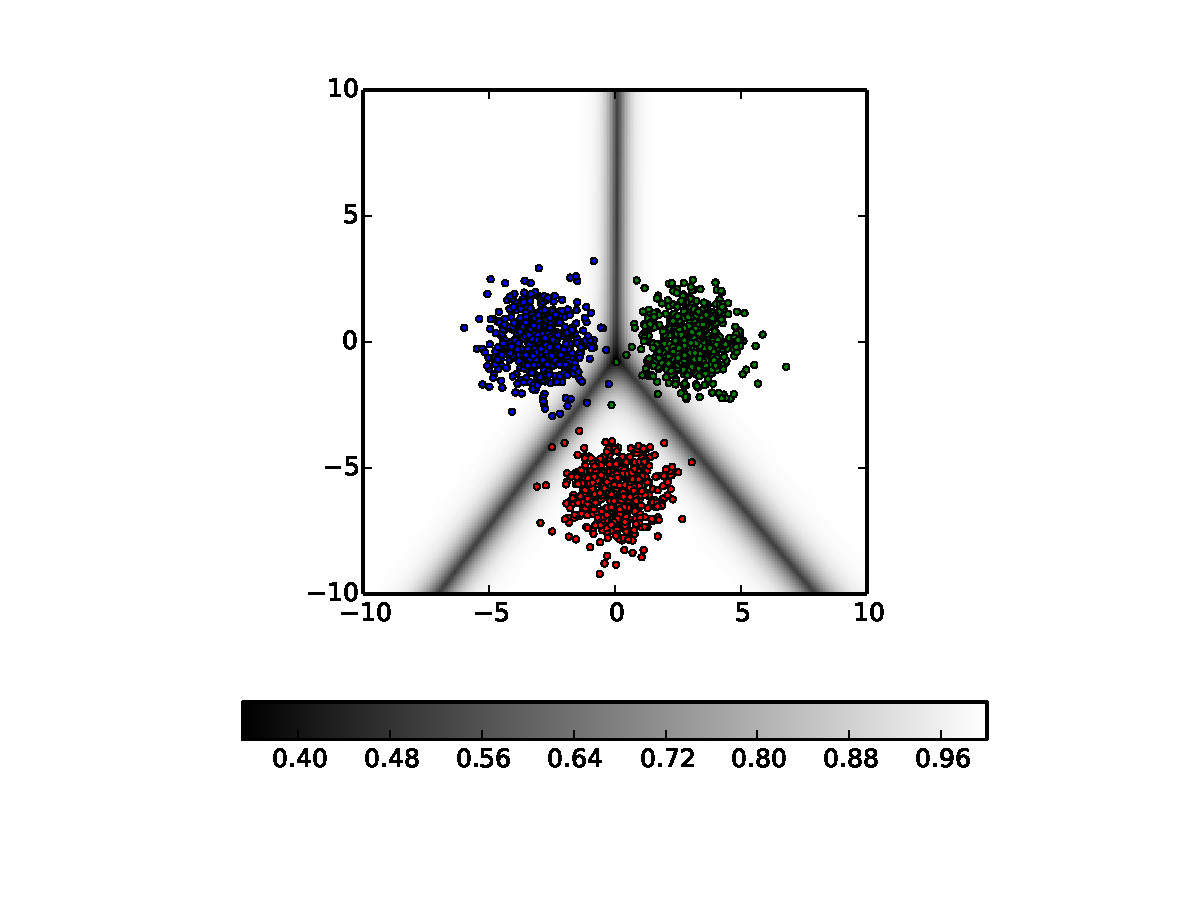
\includegraphics[width=0.49\textwidth, trim={3cm 0 1cm 0}]{../figures/softmax.pdf}}
\subfigure[GLVQ]{
 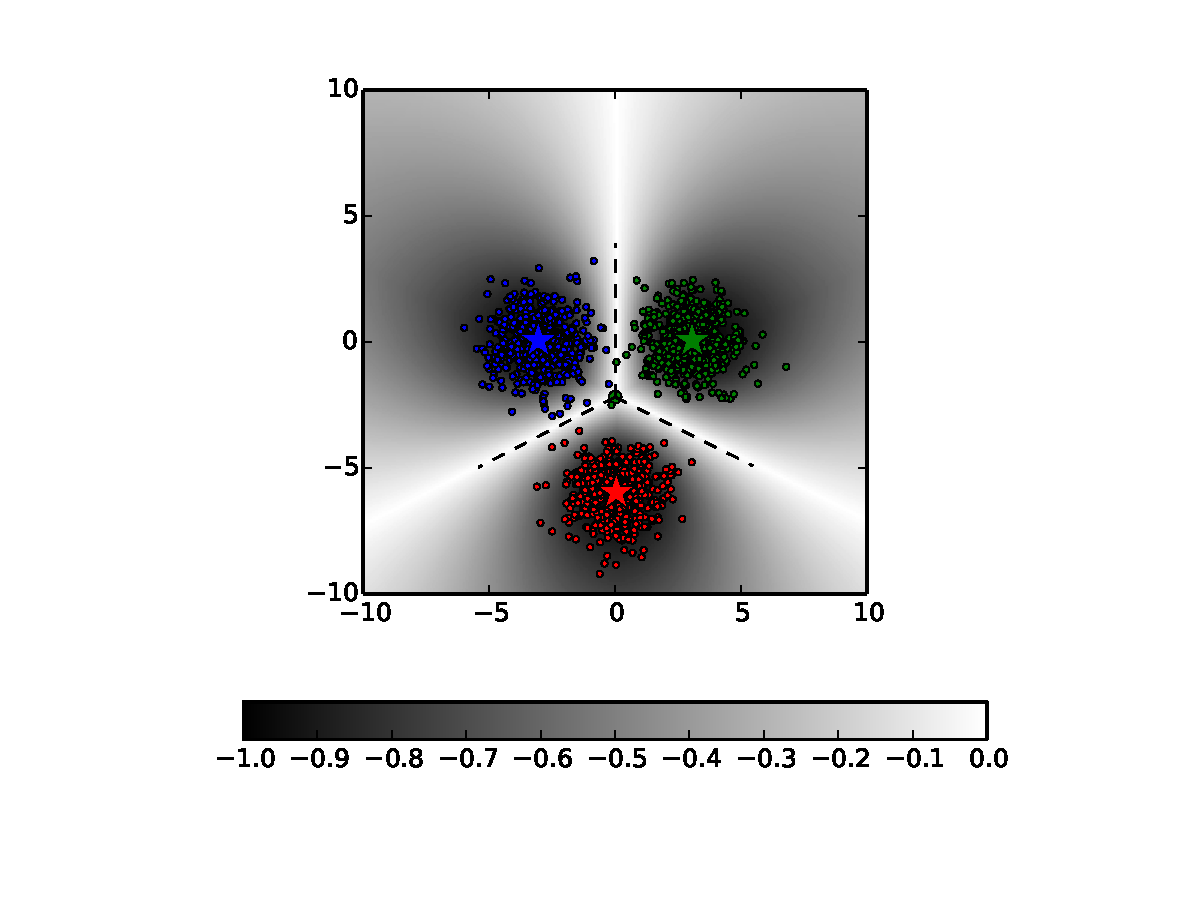
\includegraphics[width=0.49\textwidth, trim={3cm 0 1cm 0}]{../figures/lvq.pdf}}}
\caption{An artifically generated three class problem for which we have trained (a) a softmax classifier and (b) a GLVQ classifier. The background color (white for high) indicates the confidence values for a decision, that is $\mbox{arg max}_i\ p(y_j|x)$ for the softmax and $-\frac{d^{+} - d^{-}}{d^{+} + d^{-}}$\protect\footnotemark for the GLVQ classifier. The softmax classifier will assign a high confidence value to new data point in the right upper corner (far from the data), while GLVQ will not. }
\label{figure:diff_glvq_softmax}
\end{figure}

\footnotetext{We multiplied the cost with $-1$ such that higher values indicates higher confidence.}

\section{Deep GLVQ}
We propose to extend the GLVQ cost function by parameterizing the distance function as:
\begin{equation}
 d(x, w_j) = \|f(\mathbf{x}; \theta) - \mathbf{w}_j\|_2
\end{equation}
where $f$ is a deep neural network with parameters $\mathbf{\theta}$. 


\section{Related work}


\section{Experiments}
We present preliminary experiments on MNIST. 

\subsection{MNIST}
We use a fully connected neural network with $1200-1200-100$ hidden units, followed by either a softmax or GLVQ. All units have RELU activation functions. The networks are trained with batch normalization \cite{DBLP:journals/corr/IoffeS15}, and gaussian noise on the inputs. (Although a bit cheating, we trained both networks with early stopping on the training set. The softmax network obtains $0.99$ test error, and the GLVQ network $0.85$. Hyperparameters should be explored on the cluster to see the real performance. )   

\subsubsection{Adversarial examples}
We illustrate the confidence values for 

\begin{figure}[ht]
\centering{
\subfigure[Softmax]{
 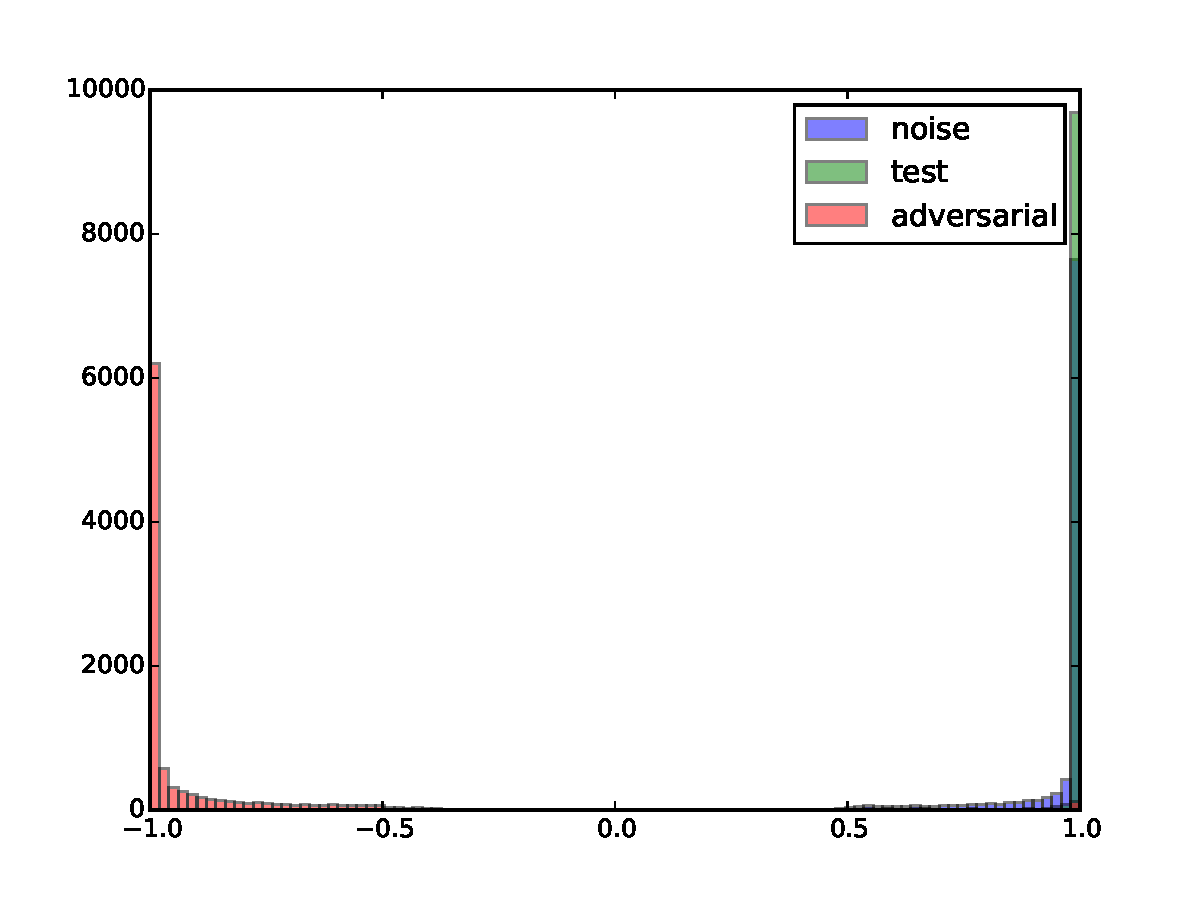
\includegraphics[width=0.49\textwidth]{../figures/softmax_conf.pdf}}
\subfigure[GLVQ]{
 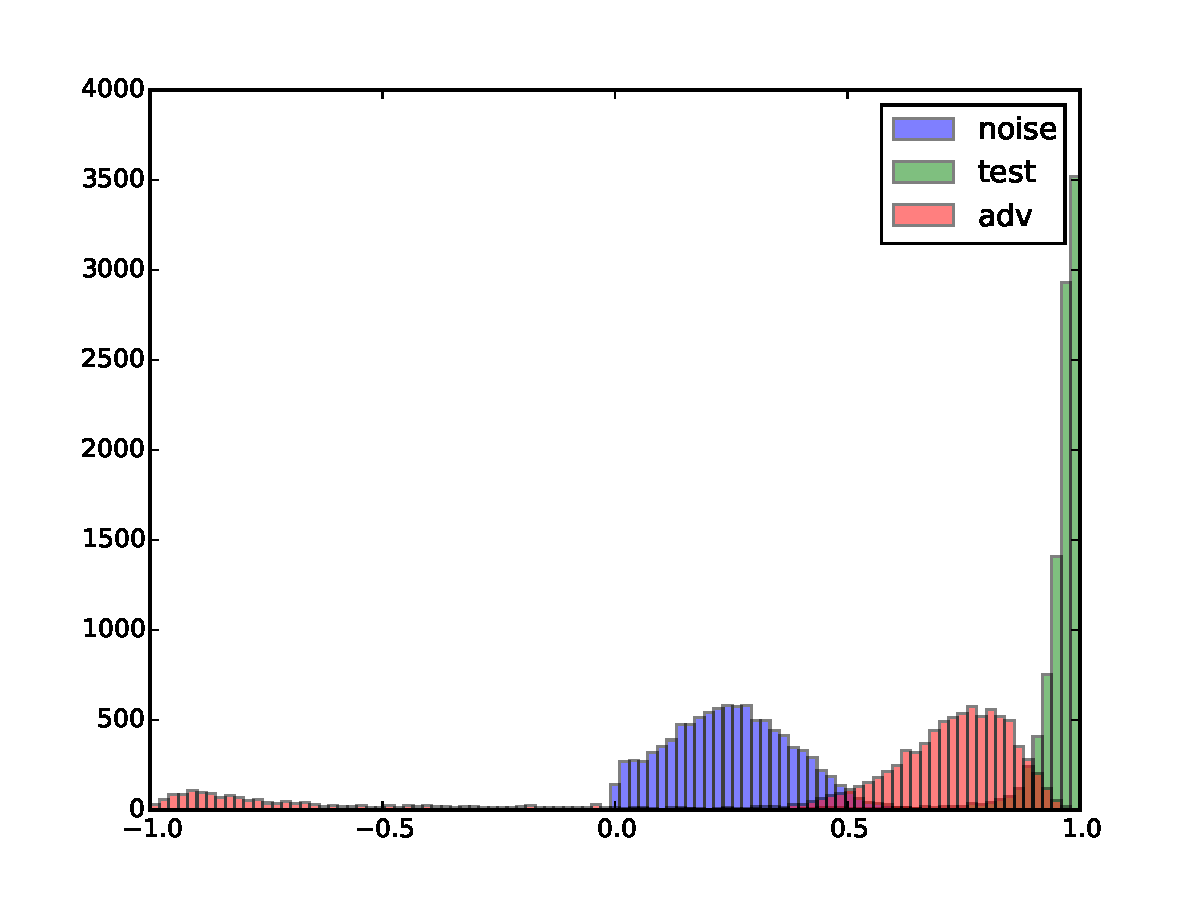
\includegraphics[width=0.49\textwidth]{../figures/lvq_conf.pdf}}}
\caption{Histogram of the confidence values for the neural network trained with a) softmax and b) GLVQ on MNIST. The green bars indicate the confidence values for the test set, the blue bars indicate the confidence values for noise drawn from $\mathcal{U}(0.0, 1.0)^{784}$ and the red bars denote the confidence for adversarial examples on the test set. }
\end{figure}

\subsubsection{Visualization of embedding}
We compare the final $100$-dimensional embedding learned by the softmax and GLVQ. To this end, we perform and eigendecomposition on the feature embeddings of both the softmax and GLVQ. The resulting eigenspectrum are plotted in Fig. \ref{figure:eigenspectrum}. As we can see, GLVQ only uses $9$ dimensions, while discarding all other dimensions. In contrast, there is a heavy tail in the distribution of eigenvalues for the softmax. At least $40$ dimensions are needed to retain most of the information. 
 
\begin{figure}[ht]
\centering{
\subfigure[Softmax]{
 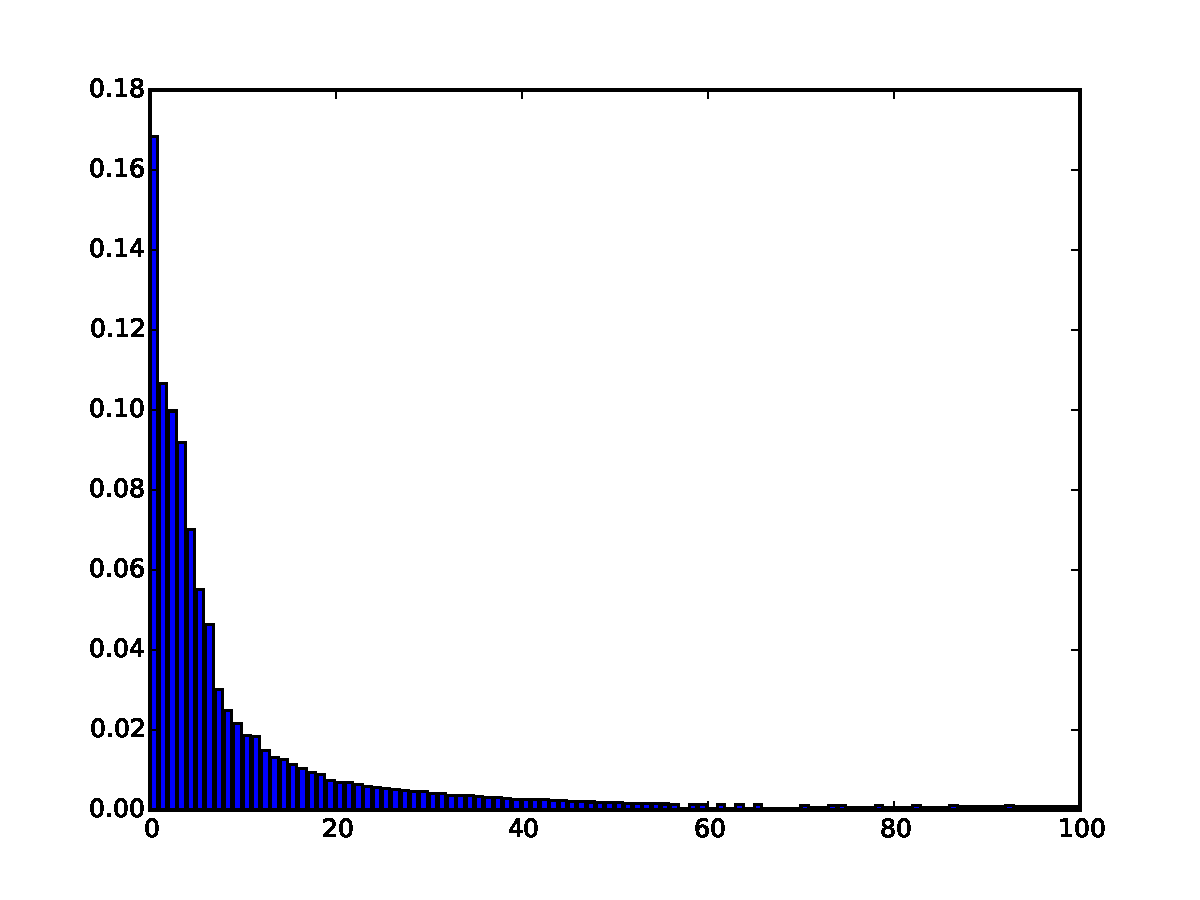
\includegraphics[width=0.49\textwidth]{../figures/softmax_embedding.pdf}}
\subfigure[GLVQ]{
 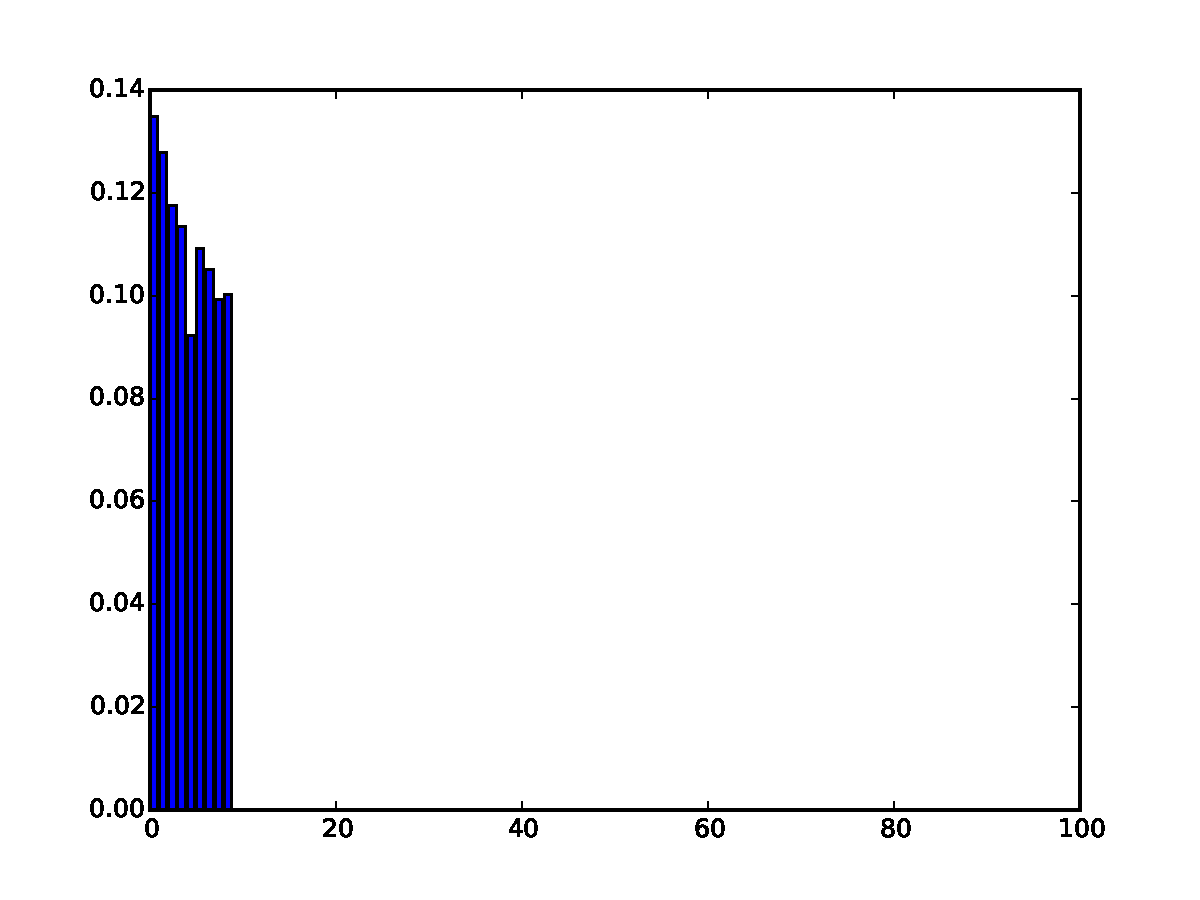
\includegraphics[width=0.49\textwidth]{../figures/lvq_embedding.pdf}}}
\caption{Histogram of the eigenvalues of the $100$-dimensional embedding of the training data. }
\label{figure:eigenspectrum}
\end{figure}

We also demonstrate the qualitative difference between the embeddings by visualizing the projection on the $3$ largest principal components. 

\begin{figure}[ht]
\centering{
\subfigure[Softmax]{
 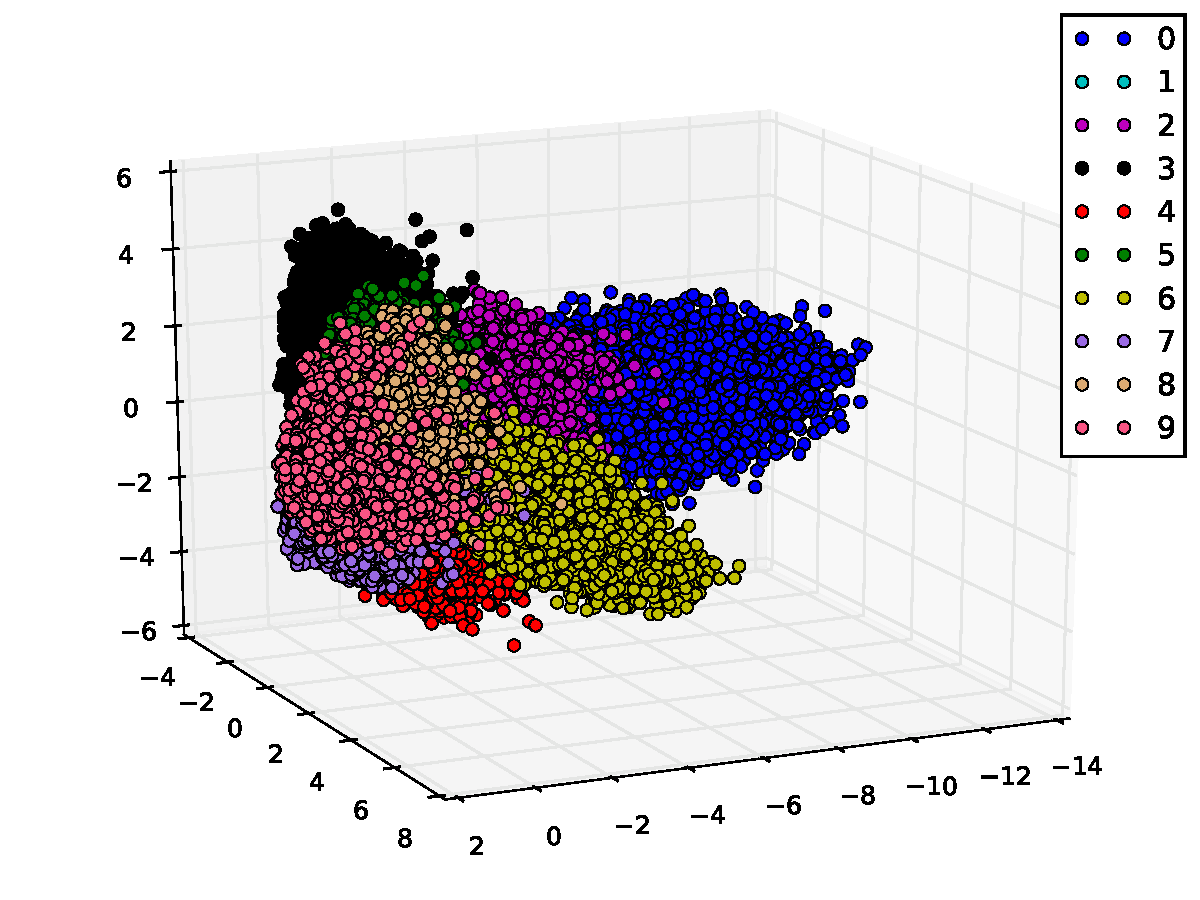
\includegraphics[width=0.49\textwidth]{../figures/softmax_embedding_3d.pdf}}
\subfigure[GLVQ]{
 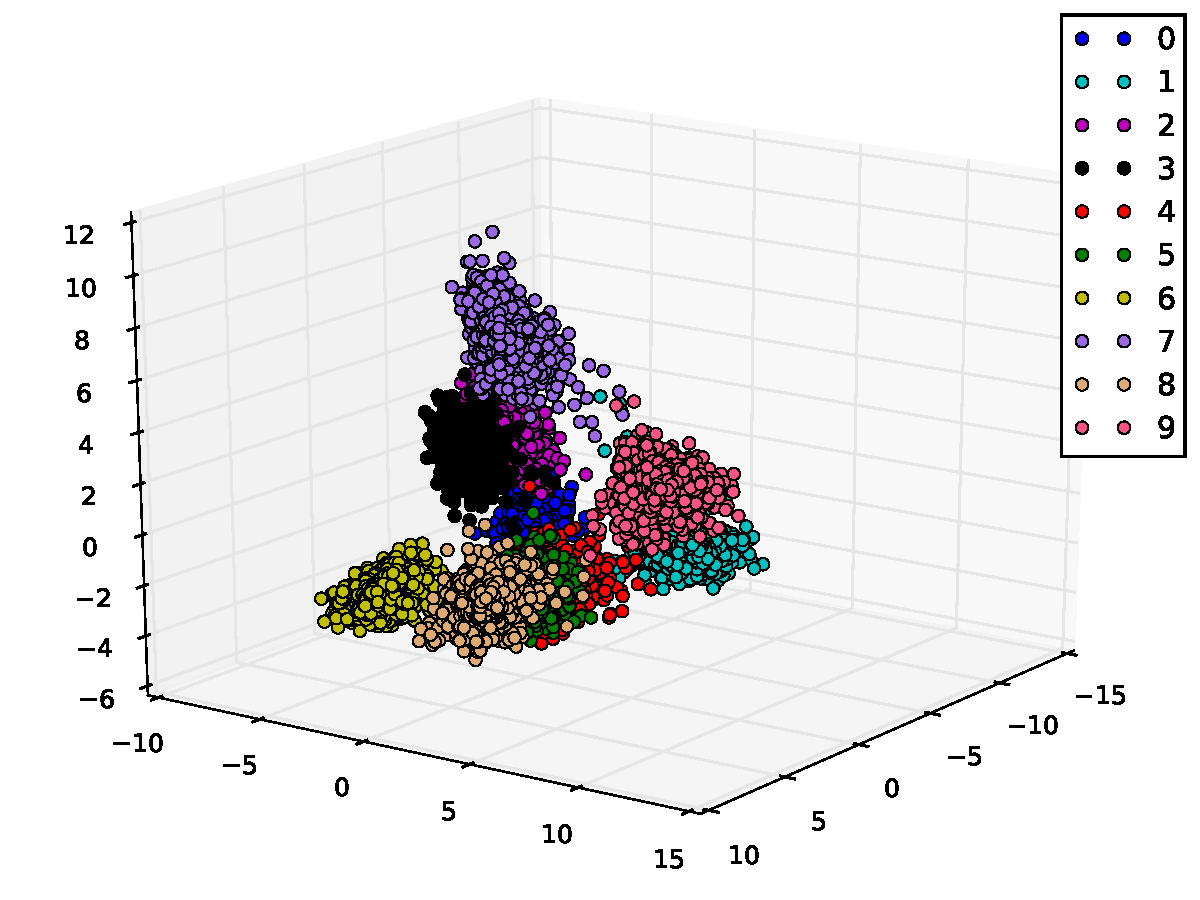
\includegraphics[width=0.49\textwidth]{../figures/lvq_embedding_3d.pdf}}}
\caption{A 3D visualization on the three largest principal components of the feature embeddings. }
\end{figure}


\subsubsection*{Acknowledgments}


\bibliography{refs}
\bibliographystyle{iclr2015}

\appendix

\section{Softmax follows from gaussian class-conditionals}
Let's assume that the class-conditional distribution $p(x|y_j) = \frac{1}{Z} \exp(-\frac{1}{2\sigma^2}(\mathbf{x} - \mathbf{w}_j)^{\top}(\mathbf{x} - \mathbf{w}_j))$ is an isotropic Gaussian distribution with normalization constant $Z = ..$. 

\end{document}
